\documentclass[conference]{IEEEtran}
\IEEEoverridecommandlockouts
% The preceding line is only needed to identify funding in the first footnote. If that is unneeded, please comment it out.
\usepackage{cite}
\usepackage{amsmath,amssymb,amsfonts}
\usepackage{algorithmic}
\usepackage{graphicx}
\usepackage{textcomp}
\usepackage{xcolor}
\usepackage{listings}
\usepackage{cuted}

\def\BibTeX{{\rm B\kern-.05em{\sc i\kern-.025em b}\kern-.08em
    T\kern-.1667em\lower.7ex\hbox{E}\kern-.125emX}}
\begin{document}

\title{Top Spotify Tracks Database}

\author{\IEEEauthorblockN{Jason Caballes}
\IEEEauthorblockA{\textit{jasoncab, SeaQwel (Team 9)} \\
\textit{CSE 560 University at Buffalo}\\
Buffalo (NY), USA \\
jasoncab@buffalo.edu}
\and
\IEEEauthorblockN{Nick Cruz}
\IEEEauthorblockA{\textit{nacruz, SeaQwel (Team 9)} \\
\textit{CSE 560 University at Buffalo}\\
Buffalo (NY), USA \\
nacruz@buffalo.edu}
\and
\IEEEauthorblockN{Utkarsh Mathur}
\IEEEauthorblockA{\textit{umathur, SeaQwel (Team 9)} \\
\textit{CSE 560 University at Buffalo}\\
Buffalo (NY), USA \\
umathur@buffalo.edu}
}
\maketitle

\begin{abstract}
Music has been a crucial component of art and society since the dawn of civilizations. The field of music and art has undergone a lot of changes over the centuries and currently our civilization at stage where we can very easily express our interests and opinions to the entire world owing to online streaming apps like Spotify \cite{b2}. Using the Spotify Web API \cite{b1} we have created a database which stores the current top 50 songs of the day for 67 countries. Our database can aid researcher and music enthusiasts across the globe analyse the current market trends and public music choice.  
\end{abstract}

\section{Introduction}
\subsection{\textbf{Task 1}: Problem Statement}
Our database system utilizes the Spotify API \cite{b1} to store the platform’s Top 50 tracks on a daily basis. The database works as a record of tracks that are currently charting across the globe. Because the system collects records daily, we prefer a database over a simple Excel file to organize the data. Furthermore, we may only be concerned with metadata related to a track, but not the track itself. A database implementation allows us to separate attributes like artist data, album data, etc. into a more organized, legible format.

\subsection{Spotify Web API \cite{b1}}
In 2017, Spotify made its Web API publicly available to aid developers and researchers by providing a wide range of functionalities. Using it, one can easily search for Spotify content; retrieve spotify metadata for artists, albums, shows, and tracks; control and interact with the playback to play and resume, seek to a position, or retrieve queue. Since its launch, Spotify API has been used by developers and researchers alike. 

\subsection{Target Users}
The primary users of this database are any music enthusiast, workers in the music industry, or any Spotify user that would like to gain more insight about songs that Spotify deems to believe are the top 50 in the world! Workers in the music industry can utilize the data provided to understand how well artists are doing over time. Workers can then understand which artists to invest in. Music enthusiasts can understand the fanbase of their favorite artists. The artist themselves can learn about their fanbase and who they typically work with when creating music! This database would most likely be used in the backend of a web or mobile application in conjunction with Spotify’s application. \linebreak This database helps in studying the behavior of masses and so it cannot be used to analyze personal music choice and preference. However, it can be used to establish certain baselines for numerous music, psycological, and social experiments. \ 

\section{Database Design}

\subsection{\textbf{Tasks 2 \& 4} - Creating Database}
We store metadata related to the daily Top 50 tracks in each country which is pulled using the Spotify Web API \cite{b1}. Each of these playlist's URLs is contained in the contries\_top\_fifty.txt file (refer to the source code). Our script sends a request to the spotify API and pulls each song's information for each of the playlist. Any entity, i.e. (Artist, Playlist, Album, Track) is an object in the form of a python dictionary. The scripts parses the data so that we can obtain tuples to populate our tables. The one issue that arised is that these objects would create non-atomic values and therefore violate 1NF. For example, an album could have multiple artists featured in it, therefore we needed to create tuples for each artist in the album.  Our script will create atomic tuples for each object that has an attribute containing multiple values. Once tuples are created, we use embedded SQL to execute our insert queries.

scripts.data\_pull\_functions.py is a python script that contains a function to pull the data for each relation we have in our database.  To upload our data we use scripts.insert\_data.py.  Each function in scripts.insert\_data.py uses the data created in the functions of scripts.data\_pull\_functions.py as an argument to upload the data to our database.

\subsection{\textbf{Task 3, 6, 7} - Database Design \& Functional Dependencies}

Our database intends to store metadata of daily Top 50 songs in each of 67 countries where Spotify is available. This means that our database would have 3350 tracks at max however the properties of these songs can prove extremely useful to researchers and music enthusiasts so designing an efficient database is required. In order to do so, we have created a database with 10 table which are interconnected through foreign keys as shown in the E/R Diagram (Fig. 1). Each of the table is in Boyce-Codd Normal Form (BCNF) owing to the Functional Dependencies associated with each table as shown below.  

\begin{figure*}
    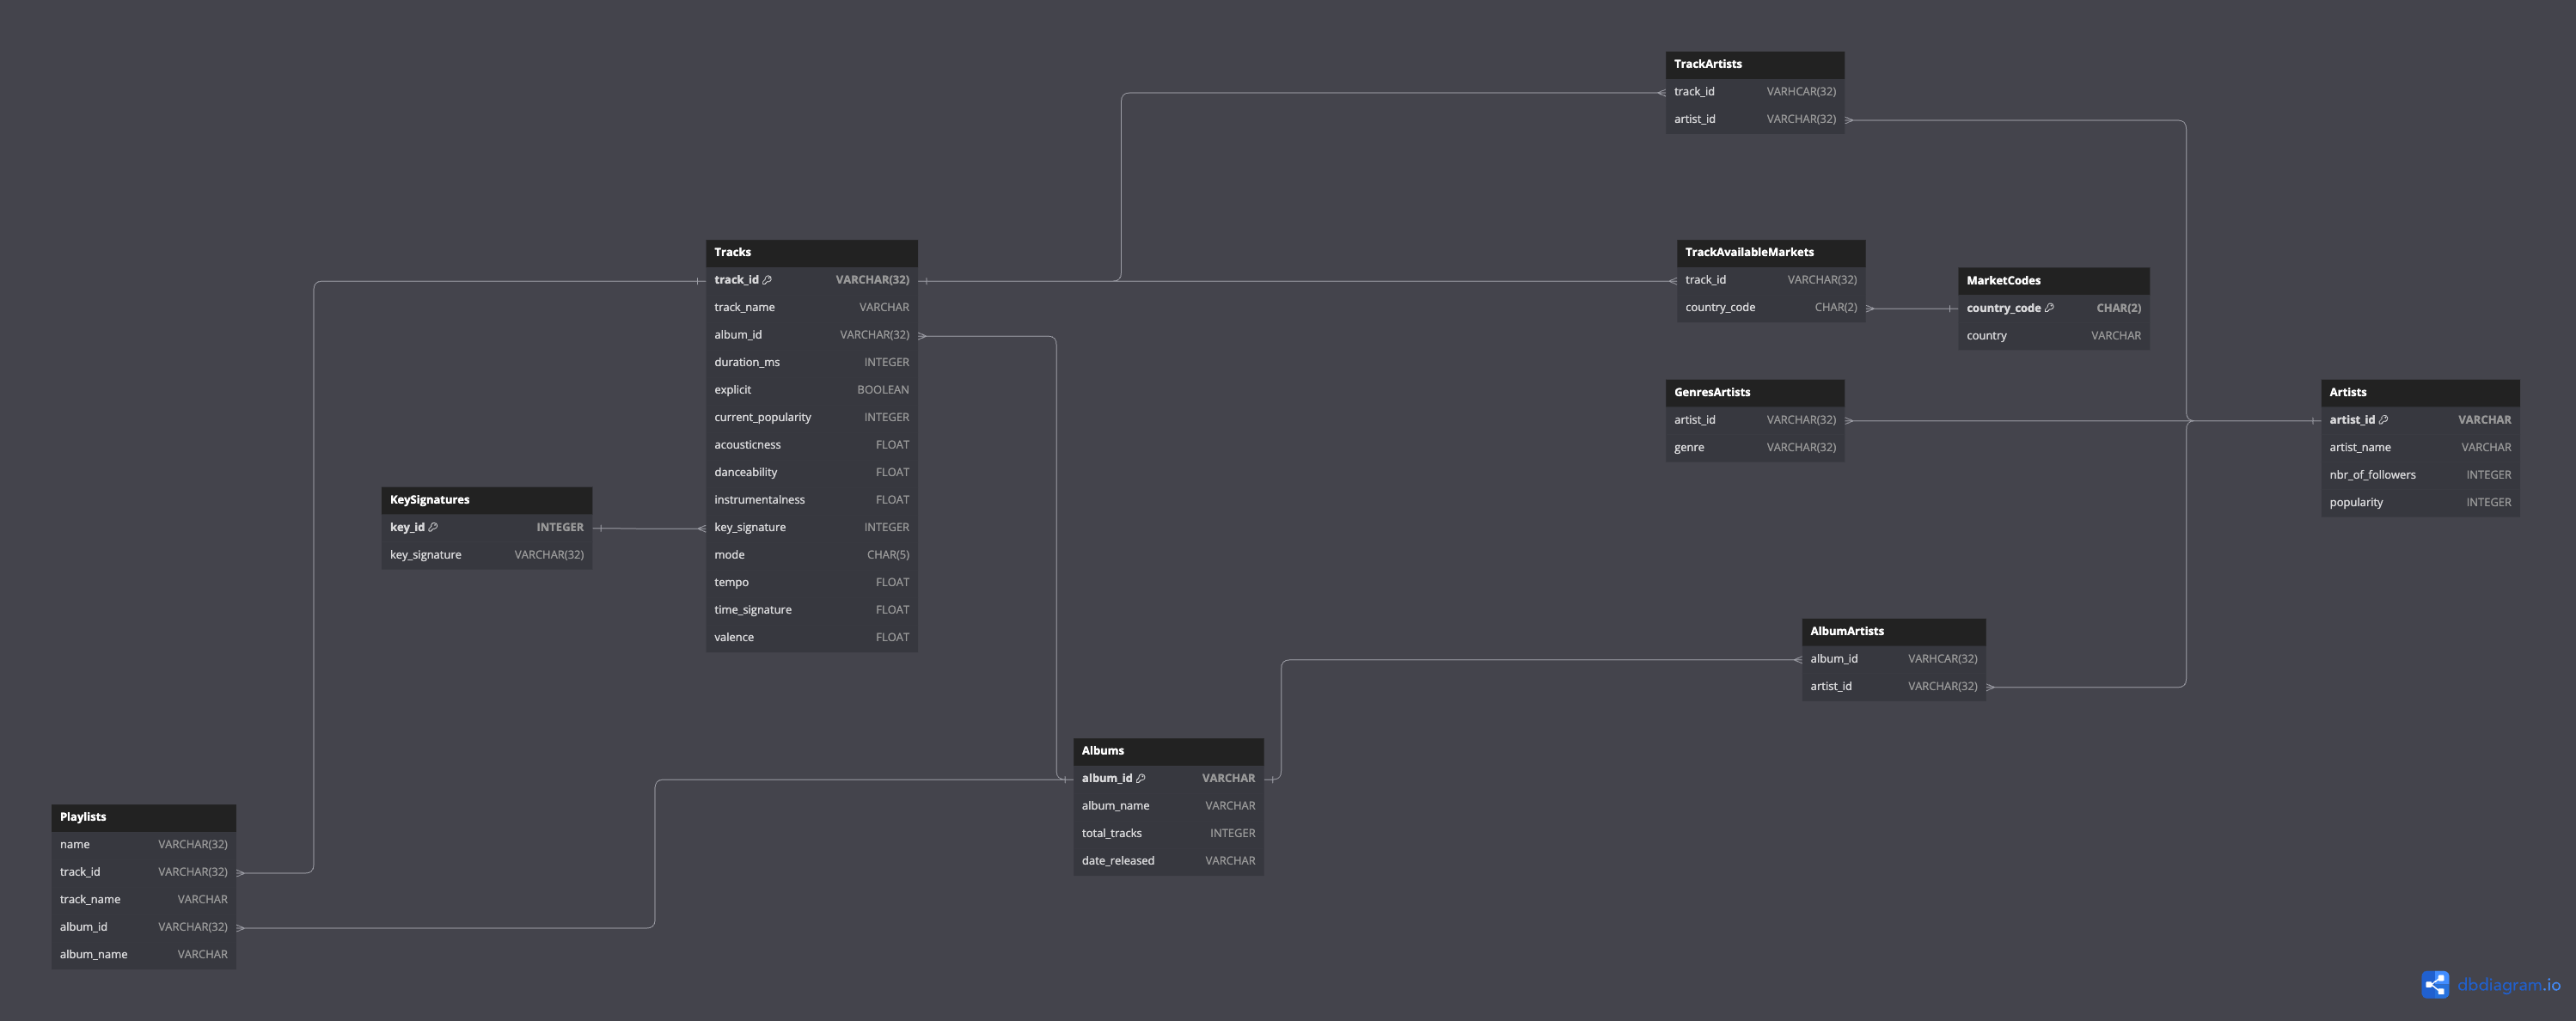
\includegraphics[width=\linewidth]{el_diagram.png}
    \caption{ER Diagram for our database}
    \label{Fig:ER Diagram}
\end{figure*}

\subsubsection*{a. \textbf{AlbumArtists} Table} \

This table stores the information about albums and the contributing artists. Since all the albums and artists have unique IDs the table only stores these IDs. \linebreak \linebreak
\textbf{AlbumID} $\to$ ArtistID \linebreak

\subsubsection*{b. \textbf{Albums} Table} \

This table stores the information regarding albums of the tracks in top 50 playlists. The table comprises of 4 attributes, i.e., AlbumID (unique ID for each album), AlbumName, TotalTracks (Total number of tracks in the album regardless their appearance in our database), and DateReleased (The date this album was released in YYYY-MM-DD format). \linebreak \linebreak
\textbf{AlbumID} $\to$ (AlbumName, TotalTracks, DateReleased) \linebreak

\subsubsection*{c. \textbf{Artists} Table} \

This table store information regarding artists features in the top 50 charts across the 67 countries. The table schema has 4 attributes - ArtistID (unique of each artist), ArtistName, NumberOfFollowers, and Popularity (a statistic designed by Spotify measuring the popularity of artists on the scale of 0-100). \linebreak \linebreak
\textbf{ArtistID} $\to$ (ArtistName, NumberOfFollowers, Popularity) \linebreak

\subsubsection*{d. \textbf{GenreArtists} Table} \

This table stores the details regarding the genres of songs produced by artists by populating two atributes - ArtistID and Genre. \linebreak \linebreak
\textbf{ArtistID} $\to$ Genre \linebreak


\subsubsection*{e. \textbf{KeySignatures} Table} \

This table stores key signature information and it is one of the 2 tables that is pre-populated. Each song has a base key around which it's music is constructed. As there is a fixed set of keys in western music notation, it is convenient to design this table. \linebreak \linebreak
\textbf{KeyID} $\to$ KeySignature \linebreak


\subsubsection*{f. \textbf{MarketCodes} Table} \

This table stores information countries regarding by assigning each Country a unique CountryCode. Fixing these CountryCodes reduced the time required to populate the table and hence this table is also pre-populated like \textbf{KeySignatures} table. \linebreak \linebreak  
\textbf{CountryCodes} $\to$ Country \linebreak


\subsubsection*{g. \textbf{TrackAvailableMarkets} Table} \

This table stores the information of countries in which a particular track is available to stream on Spotify. \linebreak \linebreak
\textbf{TrackID} $\to$ CountryCodes \linebreak


\subsubsection*{h. \textbf{Playlists} Table} \

This table is one of the most crucial tables for our database as it stores the information of playlists and their tracks. It has 5 attributes - Name (Playlist Name), TrackID (unique ID for tracks), TrackName (Name of the song), AlbumID (ID of the album of the track), and AlbumName (Name of the album of the track). A pair attributes [Name and TrackID] forms the primary key as it is convenient to define all the playlists and their contents. \linebreak \linebreak
\textbf{(Name, TrackID)} $\to$ (TrackName, AlbumID, AlbumName) \linebreak

\subsubsection*{i. \textbf{TrackArtists} Table} \

This table stores the information of tracks and their corresponding by populating two attributes - Track ID (unique ID for each song) and ArtistID (unique ID assigned to each Artist). \linebreak \linebreak
\textbf{TrackID} $\to$ ArtistID \linebreak


\subsubsection*{j. \textbf{Tracks} Table} \

This table is the main table where store all the metadata associated with a tracks in out playlist. This table has 14 attributes - TrackID (unique ID assigned to each song in the playlist), TrackName (name of the song), AlbumID (unique ID for the album of the song), Duration (the length of the track in miliseconds), Explicit (boolean value indicating global availability of the track across markets), CurrentPopularity (the popularity of the song on the current day), Accousticness (a metric generated by Spotify to measure the extent of use of accoustic instruments in the song), Dancebility (a metric generated by Spotify to measure the preference of song to dance upon), Intrumentalness (a metric generated by Spotify to measure the extent of use of instruments in the song), KeySignature (stores the information regarding the base key of the song), Mode, Tempo, TimeSignature, and Valence. \linebreak \linebreak
\textbf{TrackID} $\to$ (TrackName, AlbumID, Duration, Explicit, CurrentPopularity, Accousticness, Danceability, Instrumentalness, KeySignature, Mode, Temp0, TimeSignature, Valence)

\section{Database Analysis}

\subsection{\textbf{Task 5, 8, \& 9} - Large Dataset Test Queries}
We created a variety of queries that may arise in real-world applications. These queries involve a variety of clauses using where conditions, joins, aggregation functions on groups, partitions, ranking, and ordering. These queries exhibit the use-cases of our database and how researchers can leverage our database for further analysis. \ 

\subsubsection*{1} \textbf{Find artists with minimum number of followers in each genre}

This query can be used to establish a baseline for number of followers per artist for each genre featuring in the Top 50 Charts across the globe. \linebreak

\begin{lstlisting}[
           language=SQL,
           showspaces=false,
           basicstyle=\ttfamily,
           numbers=none,
           numberstyle=\tiny,
           commentstyle=\color{gray}
        ]
SELECT genre, 
MIN(nbr_of_followers) min_followers
FROM genreartists 
NATURAL JOIN artists 
GROUP BY genre
\end{lstlisting} \ 

\subsubsection*{2} \textbf{Find the number of countries charted for each track}

This query (and similar versions) can help researchers analyse the reach of different forms of music with respect to the number of countries tracks where they are charted. It can be crucial in understanding the music tastes of people around the globe. \linebreak  

\begin{lstlisting}[
           language=SQL,
           showspaces=false,
           basicstyle=\ttfamily,
           numbers=none,
           numberstyle=\tiny,
           commentstyle=\color{gray}
        ]
SELECT playlists.track_id,'
playlists.track_name,
COUNT(playlists.name) AS num_countries
FROM playlists
JOIN tracks ON playlists.track_id=tracks.track_id
GROUP BY (playlists.track_id,playlists.track_name)
ORDER BY num_countries DESC
\end{lstlisting} \ 

\subsubsection*{3} \textbf{Find all tracks created in 2023}

This query (along with its reditions) can be used to study the impact of songs on the audience by measuring the time they have featured on the Top 50 charts. It can further lead to understand the mood or the demand of type of music that is prefered by the audiences around the world. \linebreak  

\begin{lstlisting}[
           language=SQL,
           showspaces=false,
           basicstyle=\ttfamily,
           numbers=none,
           commentstyle=\color{gray}
        ]
SELECT * FROM tracks
JOIN albums ON tracks.album_id=albums.album_id
WHERE LEFT(ALBUMS.date_released, 4) = '2023'
\end{lstlisting} \ 

\subsubsection*{4} \textbf{Find the most popular artist for an album for every year}

These type of queries can help researchers and analyst understand and figure out the impact-full artists as well as albums per year. \linebreak

\begin{lstlisting}[
           language=SQL,
           showspaces=false,
           basicstyle=\ttfamily,
           numbers=none,
           numberstyle=\tiny,
           commentstyle=\color{gray}
        ]
WITH data AS(
SELECT AA.ALBUM_ID,AA.artist_id,
artists.artist_name, albums.album_name, 
CAST(LEFT(albums.date_released, 4) AS INT) 
AS year_released, artists.popularity,
MAX(Artists.popularity) 
OVER (PARTITION BY aa.album_id) AS
max_popularity_in_album
FROM albumartists AS AA
JOIN Albums ON AA.album_id=Albums.album_id
JOIN Artists ON AA.artist_id=Artists.artist_id)
SELECT DISTINCT album_name, 
artist_name,popularity,
year_released
FROM data
WHERE popularity = max_popularity_in_album
ORDER BY year_released DESC, album_name;
\end{lstlisting} \ 

\subsubsection*{5} \textbf{Ranks artists by popularity for every year}

This query is similar to the previous query in the sense that it too can be used to analyze the imapctfullness of artists over the year. \linebreak

\begin{lstlisting}[
           language=SQL,
           showspaces=false,
           basicstyle=\ttfamily,
           numbers=none,
           numberstyle=\tiny,
           commentstyle=\color{gray}
        ]
SELECT DISTINCT artist_name, 
year, popularity, 
DENSE_RANK() 
OVER(PARTITION BY YEAR 
ORDER BY popularity DESC) 
AS popularity_rank
FROM (SELECT *,
LEFT(ALBUMS.date_released, 4) AS year
FROM AlbumArtists
JOIN Albums 
ON AlbumArtists.album_id=Albums.album_id
JOIN Artists ON 
AlbumArtists.artist_id=Artists.artist_id) 
AS album_join_artist
ORDER BY year DESC, popularity_RANK
\end{lstlisting} \ 

\subsubsection*{6} \textbf{Find all available tracks in the United States}

This queries can be used to study the mood and music taste of audiences in a country or region. These analysis can be extremely valuable to artists, producers, and researcher alike. \linebreak 

\begin{lstlisting}[
           language=SQL,
           showspaces=false,
           basicstyle=\ttfamily,
           numbers=none,
           numberstyle=\tiny,
           commentstyle=\color{gray}
        ]
SELECT Tracks.* 
FROM Tracks
JOIN trackavailablemarkets AS markets
ON markets.track_id = Tracks.track_id
WHERE markets.country_code =
(SELECT country_code
FROM marketcodes
WHERE country = 'United States of America')
ORDER BY Tracks.track_id;
\end{lstlisting} \ 

\subsubsection*{7} \textbf{Get follower count, popularity, album count, track count, genre count for each artist}

This query and it's subsequent versions can be of special use to music connoisseurs, researchers, and studios in determining the top artists and music tastes in demand. It can further be used to analyze how well does artists connects with their audiences and how their fanbase changes over time. \linebreak  

\begin{lstlisting}[
           language=SQL,
           showspaces=false,
           basicstyle=\ttfamily,
           numbers=none,
           numberstyle=\tiny,
           commentstyle=\color{gray}
        ]
WITH genres AS(
SELECT DISTINCT 
artist_id,
COUNT(genre) 
OVER (partition by artist_id) AS genre_count 
FROM genreartists),
albums AS
(SELECT DISTINCT
artist_id,COUNT(album_id) 
OVER (partition by artist_id) 
AS album_count FROM albumartists),
tracks AS(
SELECT DISTINCT
artist_id ,COUNT(track_id) 
OVER (partition by artist_id) 
AS track_count FROM trackartists)
SELECT artists.*,album_count,
track_count,genre_count
FROM ARTISTS
JOIN albums ON 
albums.artist_id = artists.artist_id
JOIN tracks ON 
tracks.artist_id = artists.artist_id
JOIN genres ON 
genres.artist_id = artists.artist_id
ORDER BY track_count DESC
\end{lstlisting} \ 

\subsubsection*{8} \textbf{Find the average duration of tracks for each year}

This query can be used to study the evolution of music over time. It has been reported that over years \cite{b3} \cite{b4} \cite{b5} that the duration of the song impacts the time they are featured in charts and so this query can be used to study relationships between audience preference and length of the song. \linebreak

\begin{lstlisting}[
           language=SQL,
           showspaces=false,
           basicstyle=\ttfamily,
           numbers=none,
           numberstyle=\tiny,
           commentstyle=\color{gray}
        ]
WITH get_releases AS (
SELECT tracks.*,
albums.date_released
FROM tracks JOIN albums ON 
albums.album_id = tracks.album_id
)
SELECT LEFT(date_released, 4) 
AS year_released, 
ROUND(AVG(duration_ms), 2) AS 
avg_track_duration_ms
FROM get_releases
GROUP BY LEFT(date_released, 4)
ORDER BY LEFT(date_released, 4);
\end{lstlisting} \ 

The above 8 queries effectively summarizes the types of use-cases where this database can help researchers and music enthusiasts analyze the trends in music industry and derive insights which can be useful to researchers, artists, and production studios. These queries can also aid in refining songs before releasing the album and reproducing old songs tailored for the modern audiences. \linebreak One of the downsides of this database is that it helps in studying the behavior of masses and so it is of little use in analyzing music choice and preference at personal level. However, it can be used to establish certain baselines for music and psycological experiments.

\subsection{\textbf{Task 10} - Query Execution Analysis}

\begin{figure*}
    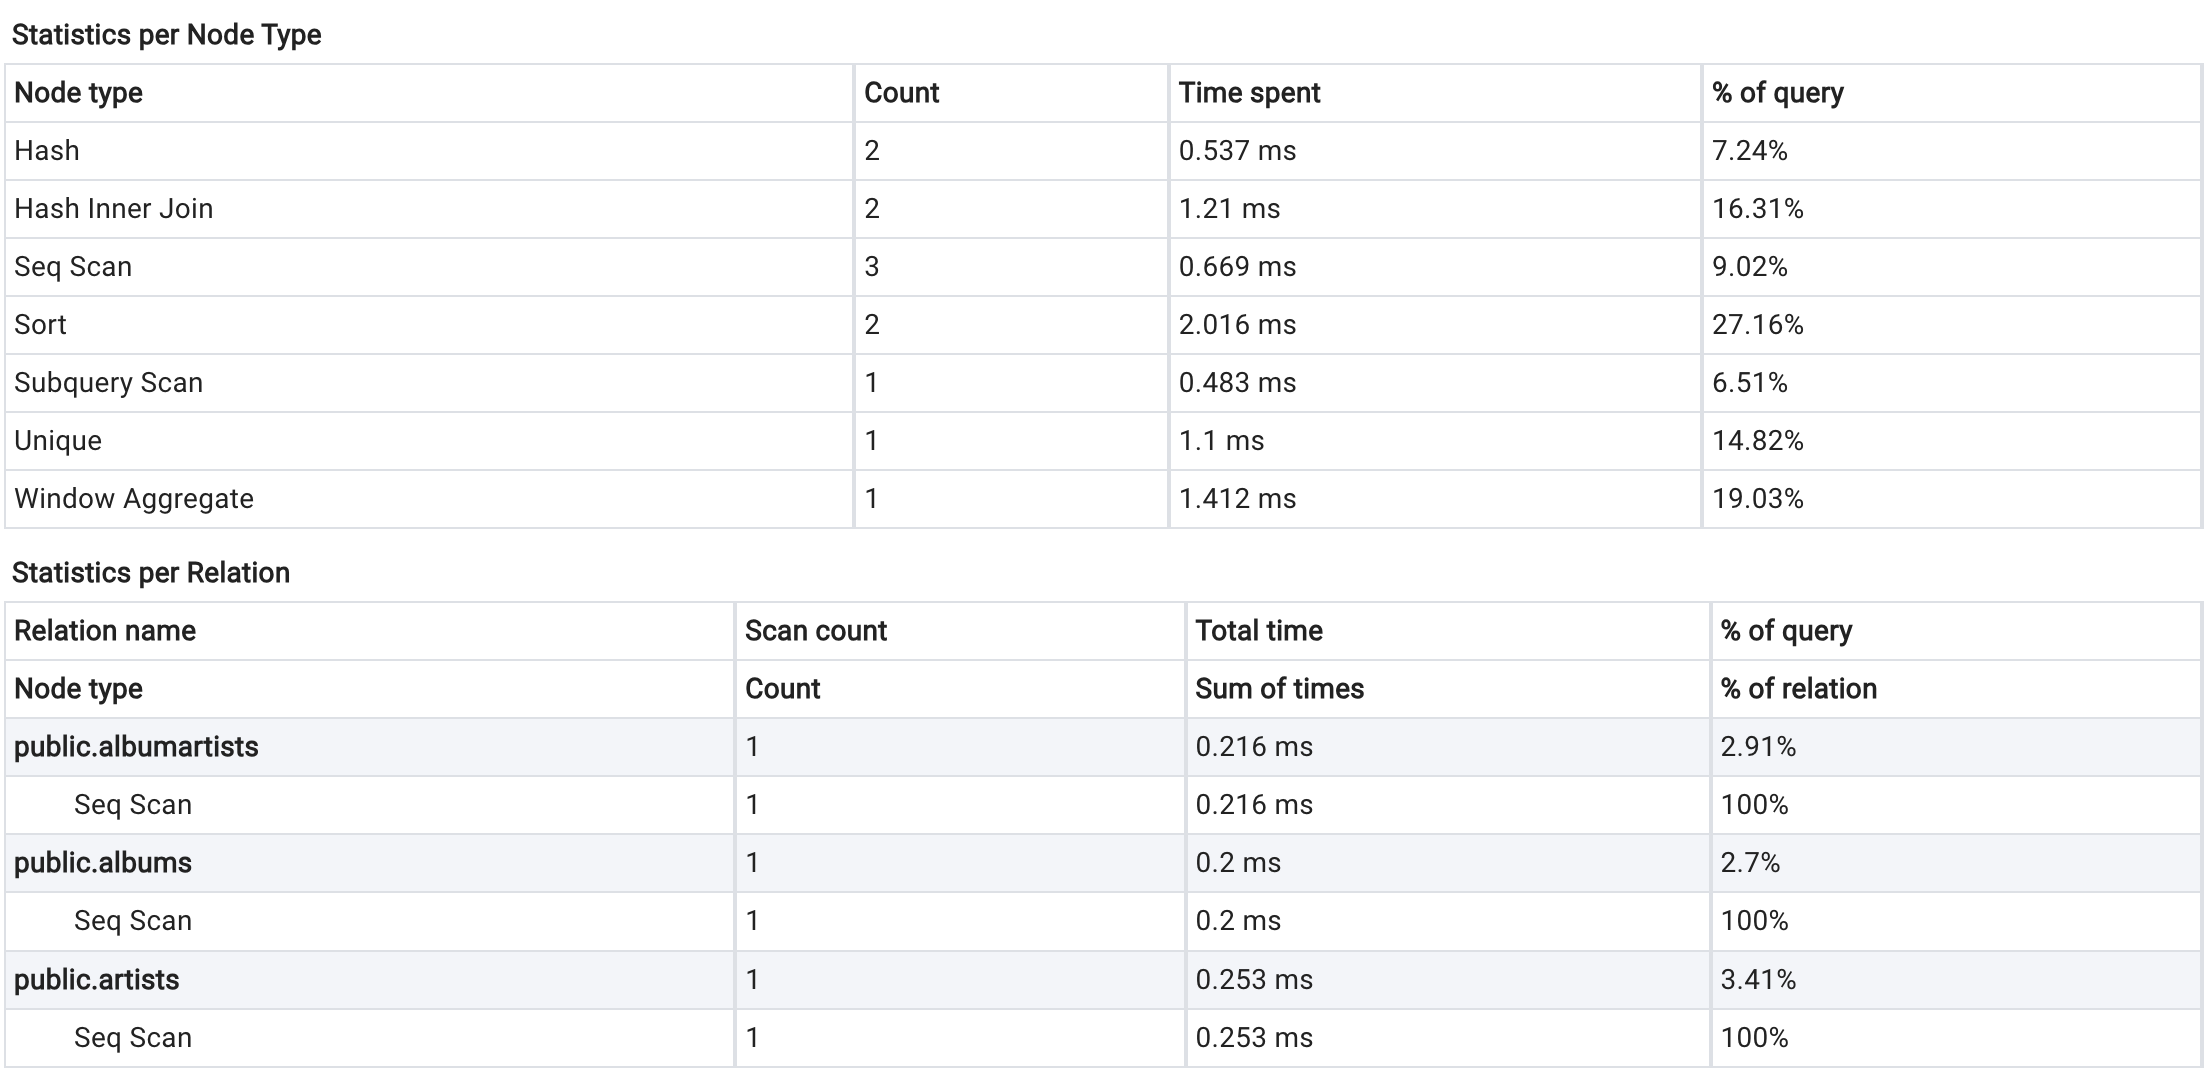
\includegraphics[scale=.41]{explain.png}
    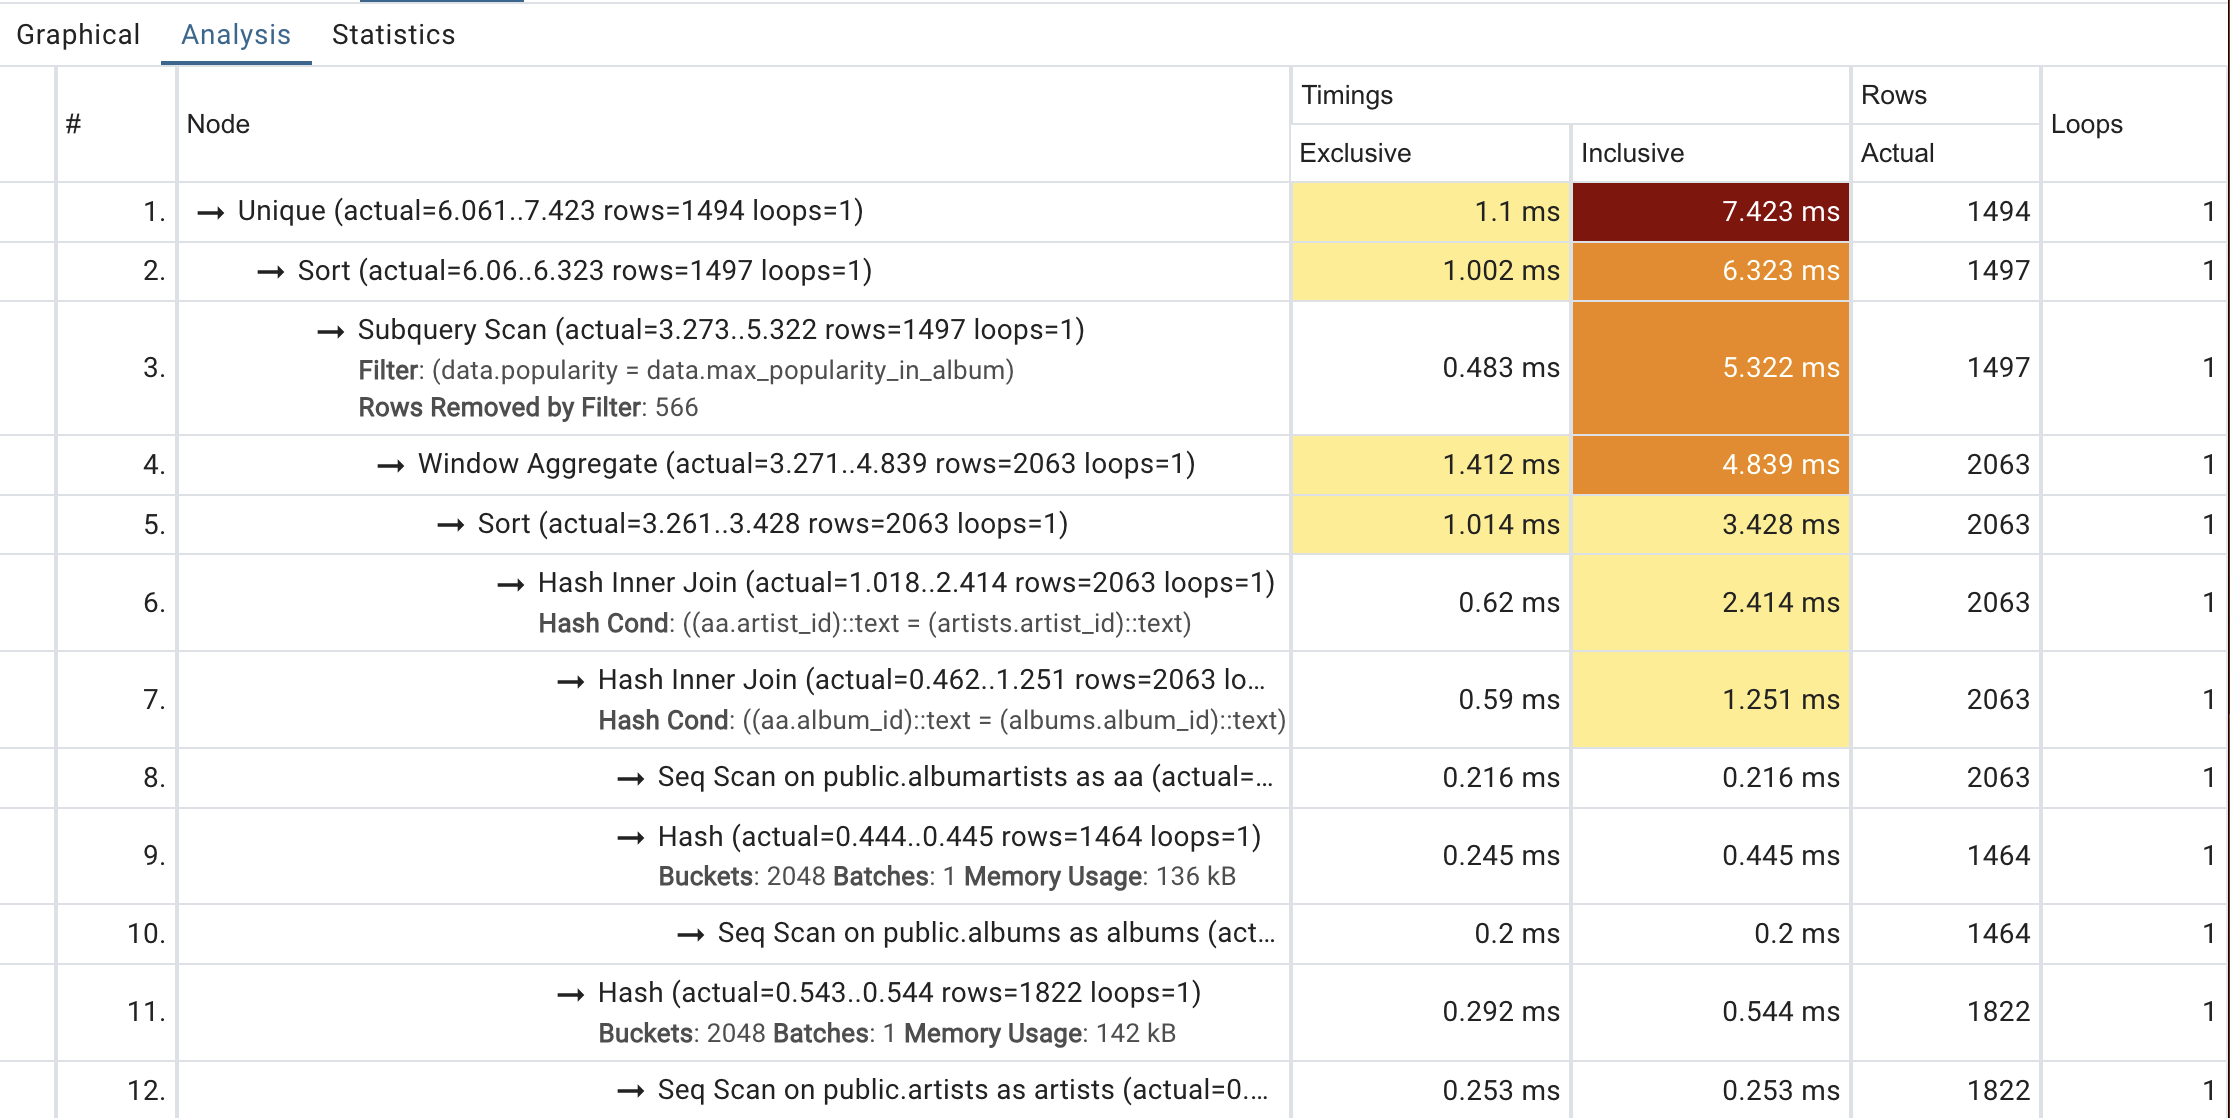
\includegraphics[scale=.40]{explain2.png}
    \caption{Explain Tool Results}
    \label{Fig:Explain Tool Results - Query 4}
\end{figure*}


Our database only has 3350 tuples in the \textbf{Playlists} relation (the largest relation of our database with respect to number of tuples), which means that our database is relatively small owing to the use-case we aim to address. Moreover, all the relations of our database are in Boyce-Codd Normal Form (BCNF) with minimal and essential foreign keys connecting the relations. By constructing the schemas meticulously we have made sure that retrieving any kind of data (within the domain of the database) should be convenient to extract and analyse. 

As an example, we have used the explain tool on a potentially problematic query, where we find the most popular artist for an album for every year (Fig. 2). This query performs multiple joins while using temporary tables. Furthermore, the query introduces more computational complexity through the \textit{max} aggregation function over a partition and through ordering the result. If the database were to scale up in size, we found that timing issues would begin to arise from joining tables on albums and artists, sorting, performing the \textit{max} aggregation function, filtering based on maximum popularity, and selecting distinct elements (Fig. 2).


\section{Conclusion}

By using the Spotify Web API \cite{b1} to extract the top 50 songs playlist of each of the 67 countries where Spotify is currently available, we are able to contruct a code base that can retrieve these playlists to populate our database. This database has 10 carefully designed relations in BCNF which are interconnected using foreign keys to allow ease of data extraction and data analysis. The database can find many application in the research of music and psycology as well as inquisitive personal projects for music enthusiasts.  


\begin{thebibliography}{00}
\bibitem{b1}Spotify, “Web API | Spotify for Developers,” developer.spotify.com. https://developer.spotify.com/documentation/web-api
\bibitem{b2}Spotify, “Spotify,” Spotify, 2024. https://open.spotify.com/
\bibitem{b3}F. Zandt, “Infographic: The Shorter the Song, the Sweeter the Stream?,” Statista Infographics, Jan. 07, 2022. https://www.statista.com/chart/26546/mean-song-duration-of-currently-streamable-songs-by-year-of-release/
\bibitem{b4}Martina, “Does The Song Length Matter?,” iMusician, Sep. 23, 2023. https://imusician.pro/en/resources/blog/does-the-song-length-matter/
\bibitem{b5}D. Sanchez, “Pop Songs Have Become Significantly Shorter Over the Past 5 Years,” Digital Music News, Jan. 18, 2019. https://www.digitalmusicnews.com/2019/01/18/streaming-music-shorter-songs-study/

\end{thebibliography}

\end{document}
